\documentclass[11pt]{article}
\usepackage[a4paper, margin=2.54cm]{geometry}

% español
\usepackage[spanish]{babel}

% imágenes
%\usepackage{graphicx}
%\graphicspath{{img}}

% fuentes de conjuntos numéricos
\usepackage{amsfonts}

% símbolos
\usepackage{amsmath, amssymb}

% gráficos
%\usepackage{tikz}

% plots
\usepackage{pgfplots}
\pgfplotsset{width=10cm, compat=1.9}

% averiguar
\setlength{\jot}{8pt}
\setlength{\parindent}{0cm}

% espacio entre párrafos
\usepackage[skip=10pt plus1pt, indent=12pt]{parskip}

% cancelar términos
\usepackage{cancel}

% links
%\usepackage[colorlinks=true, 
%    urlcolor=blue]{hyperref}

% shapes
%\usetikzlibrary{shapes.geometric}

% incluir pdfs
%\usepackage{pdfpages}

\usepackage{empheq}
\usepackage{xcolor}

\title{Economía\\Apuntes de clase\\Prof. Diego Gabriel Ramón Liut}
\author{Daniel Ise}
\date{Primer Cuatrimestre, 2025}

\begin{document}

\maketitle

\tableofcontents

\section{Carga eléctrica}

\subsection{Ley de Coulomb}

La fuerza ejercida entre cargas \(Q_1\) y \(Q_2\).

\vspace{1cm}
\begin{equation}
    F = k\frac{|Q_1Q_2|}{r^{2}}
\end{equation}
\vspace{1cm}

\begin{enumerate}
    \item Siendo F la fuerza entre las cargas (por tercera ley), medida en newton (N)
    \item \(k\) la \textbf{Constante de Coulomb} o \textbf{Constante electrostática},
    con valor aproximado 
    \begin{equation*}
        k_0\approx9\times10^{9} \frac{N\cdot m^{2}}{C^{2}}
    \end{equation*}
    \item \(Q_{1}\) y \(Q_{2}\) las cargas, medidas en coulomb (C)
    \item y \(r\) la distancia entre las mismas, medida en metros (m)
\end{enumerate}

La constante de Coulomb puede expresarse también como:

\vspace{1cm}
\begin{equation*}
    k_0 = \frac{1}{4\pi\epsilon_0}
\end{equation*}
\vspace{1cm}

Siendo \(\epsilon_0\) la \textbf{Constante de permitividad},
cuyo valor aproximado es: 
\begin{equation*}
    \epsilon_0 \approx 8.85 \times 10^{-12} \frac{C^{2}}{N\cdot m^{2}}
\end{equation*}.

\section{Campo eléctrico}

Es la fuerza potencial que una carga puede ejercer sobre una carga de prueba,
ubicada a un distancia \textit{r}.

\vspace{1cm}
\begin{equation}
    E = \frac{F}{Q_0} = k \frac{|Q|}{r^{2}}
\end{equation}
\vspace{1cm}

\begin{itemize}
    \item Siendo \(E\) el campo eléctrico, medido en \(\frac{N}{Q}\)
    \item \(F\) la fuerza que la carga \(Q\) puede potencialmente ejercer sobre la carga de prueba \(Q_0\)
    \item \(k\) la constante de Coulomb 
    \item \(r\) la distancia entre las cargas
\end{itemize}

\section{Flujo Eléctrico - Ley de Gauss}

Refiere al campo eléctrico que atraviesa una superficie de área \(A\).

\vspace{1cm}
\begin{equation*}
    \phi = E \cdot A \cdot \cos \theta
\end{equation*}
\vspace{1cm}

\begin{itemize}
    \item Siendo \(\phi\) el flujo eléctrico 
    \item \(E\) el campo eléctrico 
    \item \(A\) el área considerada
    \item \(\theta\) el ángulo entre el vector normal de la superficie y el vector del campo eléctrico
\end{itemize}

Cuando el vector normal de la superificie y el vector del campo eléctrico son paralelos,
\(\cos\theta = 1\), por lo cual la ecuación se reduce a:

\vspace{1cm}
\begin{equation}
    \phi = E\cdot A
\end{equation}
\vspace{1cm}

La ley de Gauss resulta de reemplazar \(E\) por \(k\frac{|Q|}{r^{2}}\) y,
a su vez,
\(k\) por \(\frac{1}{4\pi\epsilon_0}\).
Por otra parte,
el área considerada es la superficie de una esfera,
por lo cual \(A = 4\pi r^{2}\),
por lo cual llegamos a la expresión:

\vspace{1cm}
\begin{equation*}
    \phi = \frac{1}{4\pi\epsilon} \cdot \frac{|Q|}{r^{2}} \cdot 4\pi r^{2}
\end{equation*}
\vspace{1cm}

Simplificamos:

\vspace{1cm}
\begin{equation*}
    \phi = \frac{1}{\cancel{4\pi}\epsilon} \cdot \frac{|Q|}{\cancel{r^{2}}} \cdot \cancel{4\pi} \cancel{r^{2}}
\end{equation*}
\vspace{1cm}

Finalmente, llegamos a la expresión de la \textbf{Ley de Gauss}:

\vspace{1cm}
\begin{equation}
    \phi = \frac{|Q|}{\epsilon}
\end{equation}
\vspace{1cm}


\section{Unidad 2}

\subsection{Derivadas parciales}

La \textbf{derivada en un punto} \(P = (a,b)\),
de una función de una variable \(f(x)\),
devuelve la \textit{pendiente} \(m\),
de una recta que es tangente a \(f\) en el punto \(P\).

\vspace{.25cm}
\begin{equation*}
    \frac{df}{dx} = \lim_{\Delta x \to 0}\frac{\Delta y}{\Delta x} =
    \lim_{x \to a}\frac{f(x) - f(a)}{x-a}
\end{equation*}
\vspace{.25cm}

La derivada en funciones de dos variables sigue la misma idea:
aplicamos la derivada a cada una de las variables por separado,
considerando a la otra como constante.
Por eso hablamos de \textbf{derivada parcial}.

\begin{align*}
    \frac{\partial f}{\partial x} = f_x \\
    \\
    \frac{\partial f}{\partial y} = f_y \\
\end{align*}

Geométricamente,
podemos interpretar la derivada parcial respecto de \(x\)
en el punto \(P = (a, b, f(a,b))\),
como la \textit{pendiente} \(m\) de una recta tangente a la curva formada por
la intersección de \(f\) y el plano \(x = a\).
Lo mismo sucedería con la derivada parcial con respecto a \(y\).

\begin{figure}[H]
    \centering
    \caption{Interpretación geométrica de la derivada parcial}
    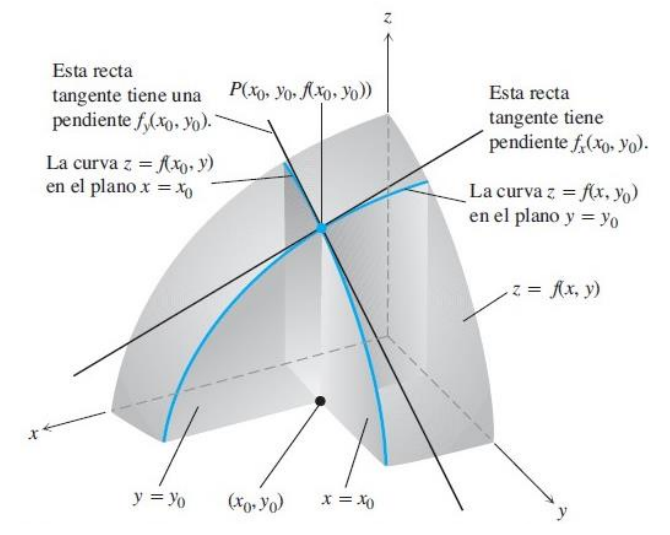
\includegraphics[scale=.8]{./img/01-02-derivada-parcial-geometrica.png}
\end{figure}

\vspace{.5cm}
\textbf{Ejemplo.}

Encontramos derivadas parciales de \(f(x,y) = x^{3} + x^{2}y^{3} - 2y^{2}\):

\begin{align*}
    f_x = 3x^{2} + 2xy^{3} \\
    f_y = 3x^{2}y^{2} - 4y \\
\end{align*}

\subsection{Propiedades y reglas de la derivada parcial}

\begin{enumerate}
    \item Con \(a\) constante:
          \begin{equation*}
              (a \cdot f)_x = a\cdot f_x
          \end{equation*}
    \item Distributiva respecto de la suma y resta:
          \begin{equation*}
              (f \pm g)_x = f_x \pm g_x
          \end{equation*}
    \item Regla del producto:
          \begin{equation*}
              (f\cdot g)_x = f_x\cdot g + f\cdot g_x
          \end{equation*}
    \item Regla del cociente:
          \begin{equation*}
              \left(\frac{f}{g}\right)_x = \frac{f_x\cdot g - f\cdot g_x}{g^{2}}
          \end{equation*}
    \item Regla de la cadena:
          Derivada parcial de \(g\), con \(f\) como está,
          por derivada parcial de \(f\):
          \begin{equation*}
              (g(f))_x = g(f)_x \cdot f_x
          \end{equation*}
\end{enumerate}

\subsection{Cálculo de derivada parcial por definición}

\subsubsection{Cuando la derivada no es continua en un punto}

Calculamos por definición,
manteniendo una constante.

\vspace{.5cm}
\textbf{Ejemplo.}

Calcular derivadas parciales de \(\sqrt[3]{x^{3} + y^{3}}\) en el origen:

Si calculamos derivada directamente:
\begin{align*}
    f_x & = \frac{1}{3}(x^{3} + y^{3})^{-2/3} \cdot 3x^{2} \\
    f_x & = \frac{x^{2}}{\sqrt[3]{(x^{3} + y^{3})^{2}}} \\
\end{align*}

Si evaluaramos esta derivada parcial en el origen,
encontraríamos una indeterminación.
Sin embargo, 
si derivamos por definición en el punto:

\begin{align*}
    f_x & = \lim_{x \to 0}\frac{f(x,0) - f(0,0)}{x - 0} \\
    f_x & = \lim_{x \to 0} \frac{\sqrt[3]{x^{3}} - 0}{x} \\
    f_x & = \boxed{1} \\
\end{align*}

Vamos con \(f_y\):

\begin{align*}
    f_y & = \lim_{y \to 0}\frac{f(0,y) - f(0,0)}{y - 0} \\
    f_y & = \lim_{y \to 0}\frac{y - 0}{y - 0} \\
    f_y & = \boxed{1}
\end{align*}

Aproximándonos por los ejes \(x\) e \(y\) la derivada tiende a \((1,1)\).


\subsubsection{Cuando está definida por partes}

Donde se da el cambio de función la derivada debe evaluarse por definición.

\vspace{.5cm}
\textbf{Ejemplo.}

Calcular derivada de:
\begin{align*}
    \begin{cases}
        \frac{3xy}{x^{2} + y^{2}} & (x,y)\neq (0,0) \\
        0 & (x,y) = (0,0)
    \end{cases}
\end{align*}

Calculamos por definición donde se produce el cambio de función:

\begin{align*}
     f_x & = \lim_{h \to 0}\frac{f(0 + h,0) - f(0,0)}{h} \\
     f_x & = \lim_{h \to 0}\frac{0 - 0}{h - 0} = \boxed{0} \\
\end{align*}

\begin{align*}
     f_y & = \lim_{h \to 0}\frac{f(0,0 + h) - f(0,0)}{h - 0} \\
     f_y & = \lim_{h \to 0}\frac{0 - 0}{h - 0} = \boxed{0} \\
\end{align*}

La derivada parcial respecto de \(x\) y respecto de \(y\) en \((0,0)\) valen 
ambas 0.

\subsubsection{Cuando puede que una exista y la otra no}

\subsubsection{Derivabilidad y continuidad}

En funciones de una variable la derivabilidad implica continuidad:
si una función es derivable en el punto \(P\),
se puede afirmar que es continua en \(P\).

Lo recíproco, siempre en funciones de una variable,
no se puede asegurar:
que una función sea continua no implica que sea derivable.
El ejemplo clásico es la función \(f(x) = |x|\). 
Esta función no es derivable en \(x = 0\),
puesto que la derivada por izquierda es distinta de la derivada por derecha.

Sin embargo,
en funciones de varias variables,
la derivabilidad \textit{no implica} continuidad.
Por ejemplo, la función \(\frac{3xy}{x^{2} + y^{2}}\).
Sus derivadas parciales en \(x\) y \(y\),
determinadas por definición,
son iguales a 0.
Pero esta función claramente \textit{no es continua} en 0.

Derivabilidad, 
en funciones de varias variables,
no implica continuidad.

\subsection{Derivadas de orden superior o derivadas sucesivas}

Una función de 2 variables independientes tiene \(2^{2}\) 
derivadas de 2\(^{\circ}\) orden:

\begin{align*}
    f_{xx} \quad f_{xy} \quad f_{yy} \quad f_{yx}
\end{align*}

Generalizando,
una función de \(m\) variables tiene \(m^{n}\) derivadas de \(n\) orden.

La notación de las derivadas de segundo orden es:

\begin{equation*}
    f_{xy} = \frac{\partial^{2} f}{\partial y \partial x} \quad 
    f_{xx} = \frac{\partial^{2} f}{\partial x^{2}}
\end{equation*}

\subsection{Teorema de Schwarz}

Si existen en torno al punto \(P\) \(f_x\),
\(f_y\)
y \(f_{xy}\),
con \(f_{xy}\) continua en \(P\),
\textbf{existe} \(f_{yx}\) y \(f_{yx}|_P = f_{xy}|_P\).

En concreto,
las derivadas cruzadas son iguales 
en todos los puntos del dominio donde sean continuas.

\vspace{.5cm}
\textbf{Ejemplo.}

Hallar derivadas de segundo orden de \(f(x,y) = x \cos y + ye^{x}\):

Hallamos primero derivadas de primer orden:

\begin{align*}
    f_x = \cos y + ye^{x} \quad f_y = -x\sen y + e^{x}
\end{align*}

Buscamos las derivadas de segundo orden:

\begin{align*}
    f_{xy} = -\sen y + e^{x} \quad f_{yx} = -\sen y + e^{x}
\end{align*}

Vemos que ambas son continuas,
por lo cual se cumple el Teorema de Schwarz:
las derivadas cruzadas son iguales.

\subsection{Dos matrices especiales}

\subsubsection{Matriz jacobiana}

Es una matriz \(m \times n\),
cuyas filas son las derivadas parciales de \(m\) funciones,
de \(n\) variables.

Por ejemplo, una matriz jacobiana de dos funciones \(f\) y \(g\),
de dos variables, sería:

\begin{equation*}
\BIG{J =
    \begin{pmatrix}
        \frac{\partial f}{\partial x} & \frac{\partial f}{\partial y} \\
        \frac{\partial g}{\partial x} & \frac{\partial g}{\partial y} \\
    \end{pmatrix}}
\end{equation*}

\subsubsection{Matriz Hessiana}

Matriz de las derivadas parciales \textit{de 2do orden}
de \textit{una} función.
Por ejemplo, la hessiana de una función de 2 variables sería:

\begin{equation*}
\BIG{H =
    \begin{pmatrix}
        f_{xx} & f_{xy} \\
        f_{yx} & f_{yy} \\
    \end{pmatrix}}
\end{equation*}

\subsection{Regla de la cadena}

Si \(f(x,y) = z\),
y podemos expresar x e y en función de t,
es decir, \(x(t)\) e \(y(t)\),
se puede hacer una composición \(z(t)\).

Se puede componer y derivar \(\frac{dz}{dt}\) o, por regla de la cadena:

\begin{equation*}
    \frac{dz}{dt} = \frac{\partial z}{\partial x}\cdot\frac{dx}{dt} + \frac{\partial z}{\partial y}\cdot\frac{dy}{dt}
\end{equation*}

Ahora, 
supongamos \(z = f(x,y)\),
que a su vez \(x = x(u,v)\) e \(y = y(u,v)\).
En este caso,
\(z\) tendrá una derivada parcial respecto de \(u\)
y una derivada parcial respecto de \(v\),
siguiendo la estructura del punto anterior:

\begin{align*}
    z_u = f_x\cdot x_u + f_y \cdot y_u \\
    z_v = f_x\cdot x_v + f_y \cdot y_v \\
\end{align*}

\subsection{Derivada direccional}

Ya hemos visto las derivadas parciales,
que son las tasas de cambio de \(z\) en dirección de los ejes \(x\) e \(y\).

La derivada direccional es la tasa de cambio del campo vectorial en dirección 
de un vector \(\vec{u}\).

El vector \(\vec{u}\) puede definirse básicamente de dos maneras:
\begin{itemize}
    \item Con \textbf{puntos} \(a\) y \(b\), 
    que para referir el vector al origen los restamos \(\vec{u} = b-a\)
    \item Con el \textbf{ángulo} \(\theta\),
    de forma \(\vec{u} = (\cos \theta, \sen \theta)\).
\end{itemize}

Para realizar una derivada direccional el vector debe estar normalizado.
Un vector dado por su ángulo \textit{ya se encuentra normalizado}.
Para normalizar un vector dado por sus puntos operamos:

\begin{equation*}
    \vec{n} = \frac{\vec{u}}{|\vec{u}|}
\end{equation*}

Siendo la magnitud del vector \(|\vec{u}| = \sqrt{a^{2} + b^{2}}\).

Dado el punto \(P = (x_0, y_0, z_0)\), 
la derivada direccional en dirección de \(\vec{u} = (a,b)\) es:

\begin{equation*}
    D_{\vec{u}}f(x,y) = \lim_{h \to 0}
    \frac{f(x_0 + ha, y_0 + hb) - f(x_0,y_0)}{h}
\end{equation*}

\textbf{Teorema de la derivada direccional.}

Si \(f\) es diferenciable en \(P = (x_0,y_0)\),
entonces tiene derivada direccional en sentido de cualquier vector 
\(\vec{u} = (a,b)\), donde:

\begin{equation*}
    D_{\vec{u}}f(x,y) = f_x|_{P} \cdot a + f_y|_{P} \cdot b
\end{equation*}

\textbf{Ejemplo.}

Hallar derivada direccional de \(f(x,y) = x^{3} - 3xy + 4y^{2}\),
en dirección de \(\vec{u}\) con \(\theta = \pi/6\).
Determinar valor de la razón de cambio siguiendo ese vector en \(P = (1,2)\).

Instrucciones:
\begin{itemize}
    \item Primero especificamos/normalizamos el vector
    \item Calculamos derivadas parciales 
    \item Planteo el teorema de la derivada direccional 
    \item Obtengo una expresión
    \item Evaluamos en \(P\)
    \item Llegamos al valor
\end{itemize}
\section{Unidad 2}

\subsection{Derivadas parciales}

La \textbf{derivada en un punto} \(P = (a,b)\),
de una función de una variable \(f(x)\),
devuelve la \textit{pendiente} \(m\),
de una recta que es tangente a \(f\) en el punto \(P\).

\vspace{.25cm}
\begin{equation*}
    \frac{df}{dx} = \lim_{\Delta x \to 0}\frac{\Delta y}{\Delta x} =
    \lim_{x \to a}\frac{f(x) - f(a)}{x-a}
\end{equation*}
\vspace{.25cm}

La derivada en funciones de dos variables sigue la misma idea:
aplicamos la derivada a cada una de las variables por separado,
considerando a la otra como constante.
Por eso hablamos de \textbf{derivada parcial}.

\begin{align*}
    \frac{\partial f}{\partial x} = f_x \\
    \\
    \frac{\partial f}{\partial y} = f_y \\
\end{align*}

Geométricamente,
podemos interpretar la derivada parcial respecto de \(x\)
en el punto \(P = (a, b, f(a,b))\),
como la \textit{pendiente} \(m\) de una recta tangente a la curva formada por
la intersección de \(f\) y el plano \(x = a\).
Lo mismo sucedería con la derivada parcial con respecto a \(y\).

\begin{figure}[H]
    \centering
    \caption{Interpretación geométrica de la derivada parcial}
    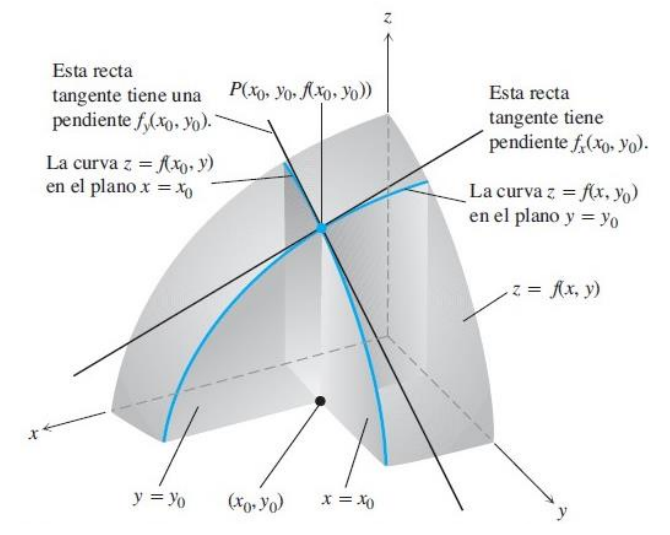
\includegraphics[scale=.8]{./img/01-02-derivada-parcial-geometrica.png}
\end{figure}

\vspace{.5cm}
\textbf{Ejemplo.}

Encontramos derivadas parciales de \(f(x,y) = x^{3} + x^{2}y^{3} - 2y^{2}\):

\begin{align*}
    f_x = 3x^{2} + 2xy^{3} \\
    f_y = 3x^{2}y^{2} - 4y \\
\end{align*}

\subsection{Propiedades y reglas de la derivada parcial}

\begin{enumerate}
    \item Con \(a\) constante:
          \begin{equation*}
              (a \cdot f)_x = a\cdot f_x
          \end{equation*}
    \item Distributiva respecto de la suma y resta:
          \begin{equation*}
              (f \pm g)_x = f_x \pm g_x
          \end{equation*}
    \item Regla del producto:
          \begin{equation*}
              (f\cdot g)_x = f_x\cdot g + f\cdot g_x
          \end{equation*}
    \item Regla del cociente:
          \begin{equation*}
              \left(\frac{f}{g}\right)_x = \frac{f_x\cdot g - f\cdot g_x}{g^{2}}
          \end{equation*}
    \item Regla de la cadena:
          Derivada parcial de \(g\), con \(f\) como está,
          por derivada parcial de \(f\):
          \begin{equation*}
              (g(f))_x = g(f)_x \cdot f_x
          \end{equation*}
\end{enumerate}

\subsection{Cálculo de derivada parcial por definición}

\subsubsection{Cuando la derivada no es continua en un punto}

Calculamos por definición,
manteniendo una constante.

\vspace{.5cm}
\textbf{Ejemplo.}

Calcular derivadas parciales de \(\sqrt[3]{x^{3} + y^{3}}\) en el origen:

Si calculamos derivada directamente:
\begin{align*}
    f_x & = \frac{1}{3}(x^{3} + y^{3})^{-2/3} \cdot 3x^{2} \\
    f_x & = \frac{x^{2}}{\sqrt[3]{(x^{3} + y^{3})^{2}}} \\
\end{align*}

Si evaluaramos esta derivada parcial en el origen,
encontraríamos una indeterminación.
Sin embargo, 
si derivamos por definición en el punto:

\begin{align*}
    f_x & = \lim_{x \to 0}\frac{f(x,0) - f(0,0)}{x - 0} \\
    f_x & = \lim_{x \to 0} \frac{\sqrt[3]{x^{3}} - 0}{x} \\
    f_x & = \boxed{1} \\
\end{align*}

Vamos con \(f_y\):

\begin{align*}
    f_y & = \lim_{y \to 0}\frac{f(0,y) - f(0,0)}{y - 0} \\
    f_y & = \lim_{y \to 0}\frac{y - 0}{y - 0} \\
    f_y & = \boxed{1}
\end{align*}

Aproximándonos por los ejes \(x\) e \(y\) la derivada tiende a \((1,1)\).


\subsubsection{Cuando está definida por partes}

Donde se da el cambio de función la derivada debe evaluarse por definición.

\vspace{.5cm}
\textbf{Ejemplo.}

Calcular derivada de:
\begin{align*}
    \begin{cases}
        \frac{3xy}{x^{2} + y^{2}} & (x,y)\neq (0,0) \\
        0 & (x,y) = (0,0)
    \end{cases}
\end{align*}

Calculamos por definición donde se produce el cambio de función:

\begin{align*}
     f_x & = \lim_{h \to 0}\frac{f(0 + h,0) - f(0,0)}{h} \\
     f_x & = \lim_{h \to 0}\frac{0 - 0}{h - 0} = \boxed{0} \\
\end{align*}

\begin{align*}
     f_y & = \lim_{h \to 0}\frac{f(0,0 + h) - f(0,0)}{h - 0} \\
     f_y & = \lim_{h \to 0}\frac{0 - 0}{h - 0} = \boxed{0} \\
\end{align*}

La derivada parcial respecto de \(x\) y respecto de \(y\) en \((0,0)\) valen 
ambas 0.

\subsubsection{Cuando puede que una exista y la otra no}

\subsubsection{Derivabilidad y continuidad}

En funciones de una variable la derivabilidad implica continuidad:
si una función es derivable en el punto \(P\),
se puede afirmar que es continua en \(P\).

Lo recíproco, siempre en funciones de una variable,
no se puede asegurar:
que una función sea continua no implica que sea derivable.
El ejemplo clásico es la función \(f(x) = |x|\). 
Esta función no es derivable en \(x = 0\),
puesto que la derivada por izquierda es distinta de la derivada por derecha.

Sin embargo,
en funciones de varias variables,
la derivabilidad \textit{no implica} continuidad.
Por ejemplo, la función \(\frac{3xy}{x^{2} + y^{2}}\).
Sus derivadas parciales en \(x\) y \(y\),
determinadas por definición,
son iguales a 0.
Pero esta función claramente \textit{no es continua} en 0.

Derivabilidad, 
en funciones de varias variables,
no implica continuidad.

\subsection{Derivadas de orden superior o derivadas sucesivas}

Una función de 2 variables independientes tiene \(2^{2}\) 
derivadas de 2\(^{\circ}\) orden:

\begin{align*}
    f_{xx} \quad f_{xy} \quad f_{yy} \quad f_{yx}
\end{align*}

Generalizando,
una función de \(m\) variables tiene \(m^{n}\) derivadas de \(n\) orden.

La notación de las derivadas de segundo orden es:

\begin{equation*}
    f_{xy} = \frac{\partial^{2} f}{\partial y \partial x} \quad 
    f_{xx} = \frac{\partial^{2} f}{\partial x^{2}}
\end{equation*}

\subsection{Teorema de Schwarz}

Si existen en torno al punto \(P\) \(f_x\),
\(f_y\)
y \(f_{xy}\),
con \(f_{xy}\) continua en \(P\),
\textbf{existe} \(f_{yx}\) y \(f_{yx}|_P = f_{xy}|_P\).

En concreto,
las derivadas cruzadas son iguales 
en todos los puntos del dominio donde sean continuas.

\vspace{.5cm}
\textbf{Ejemplo.}

Hallar derivadas de segundo orden de \(f(x,y) = x \cos y + ye^{x}\):

Hallamos primero derivadas de primer orden:

\begin{align*}
    f_x = \cos y + ye^{x} \quad f_y = -x\sen y + e^{x}
\end{align*}

Buscamos las derivadas de segundo orden:

\begin{align*}
    f_{xy} = -\sen y + e^{x} \quad f_{yx} = -\sen y + e^{x}
\end{align*}

Vemos que ambas son continuas,
por lo cual se cumple el Teorema de Schwarz:
las derivadas cruzadas son iguales.

\subsection{Dos matrices especiales}

\subsubsection{Matriz jacobiana}

Es una matriz \(m \times n\),
cuyas filas son las derivadas parciales de \(m\) funciones,
de \(n\) variables.

Por ejemplo, una matriz jacobiana de dos funciones \(f\) y \(g\),
de dos variables, sería:

\begin{equation*}
\BIG{J =
    \begin{pmatrix}
        \frac{\partial f}{\partial x} & \frac{\partial f}{\partial y} \\
        \frac{\partial g}{\partial x} & \frac{\partial g}{\partial y} \\
    \end{pmatrix}}
\end{equation*}

\subsubsection{Matriz Hessiana}

Matriz de las derivadas parciales \textit{de 2do orden}
de \textit{una} función.
Por ejemplo, la hessiana de una función de 2 variables sería:

\begin{equation*}
\BIG{H =
    \begin{pmatrix}
        f_{xx} & f_{xy} \\
        f_{yx} & f_{yy} \\
    \end{pmatrix}}
\end{equation*}

\subsection{Regla de la cadena}

Si \(f(x,y) = z\),
y podemos expresar x e y en función de t,
es decir, \(x(t)\) e \(y(t)\),
se puede hacer una composición \(z(t)\).

Se puede componer y derivar \(\frac{dz}{dt}\) o, por regla de la cadena:

\begin{equation*}
    \frac{dz}{dt} = \frac{\partial z}{\partial x}\cdot\frac{dx}{dt} + \frac{\partial z}{\partial y}\cdot\frac{dy}{dt}
\end{equation*}

Ahora, 
supongamos \(z = f(x,y)\),
que a su vez \(x = x(u,v)\) e \(y = y(u,v)\).
En este caso,
\(z\) tendrá una derivada parcial respecto de \(u\)
y una derivada parcial respecto de \(v\),
siguiendo la estructura del punto anterior:

\begin{align*}
    z_u = f_x\cdot x_u + f_y \cdot y_u \\
    z_v = f_x\cdot x_v + f_y \cdot y_v \\
\end{align*}

\subsection{Derivada direccional}

Ya hemos visto las derivadas parciales,
que son las tasas de cambio de \(z\) en dirección de los ejes \(x\) e \(y\).

La derivada direccional es la tasa de cambio del campo vectorial en dirección 
de un vector \(\vec{u}\).

El vector \(\vec{u}\) puede definirse básicamente de dos maneras:
\begin{itemize}
    \item Con \textbf{puntos} \(a\) y \(b\), 
    que para referir el vector al origen los restamos \(\vec{u} = b-a\)
    \item Con el \textbf{ángulo} \(\theta\),
    de forma \(\vec{u} = (\cos \theta, \sen \theta)\).
\end{itemize}

Para realizar una derivada direccional el vector debe estar normalizado.
Un vector dado por su ángulo \textit{ya se encuentra normalizado}.
Para normalizar un vector dado por sus puntos operamos:

\begin{equation*}
    \vec{n} = \frac{\vec{u}}{|\vec{u}|}
\end{equation*}

Siendo la magnitud del vector \(|\vec{u}| = \sqrt{a^{2} + b^{2}}\).

Dado el punto \(P = (x_0, y_0, z_0)\), 
la derivada direccional en dirección de \(\vec{u} = (a,b)\) es:

\begin{equation*}
    D_{\vec{u}}f(x,y) = \lim_{h \to 0}
    \frac{f(x_0 + ha, y_0 + hb) - f(x_0,y_0)}{h}
\end{equation*}

\textbf{Teorema de la derivada direccional.}

Si \(f\) es diferenciable en \(P = (x_0,y_0)\),
entonces tiene derivada direccional en sentido de cualquier vector 
\(\vec{u} = (a,b)\), donde:

\begin{equation*}
    D_{\vec{u}}f(x,y) = f_x|_{P} \cdot a + f_y|_{P} \cdot b
\end{equation*}

\textbf{Ejemplo.}

Hallar derivada direccional de \(f(x,y) = x^{3} - 3xy + 4y^{2}\),
en dirección de \(\vec{u}\) con \(\theta = \pi/6\).
Determinar valor de la razón de cambio siguiendo ese vector en \(P = (1,2)\).

Instrucciones:
\begin{itemize}
    \item Primero especificamos/normalizamos el vector
    \item Calculamos derivadas parciales 
    \item Planteo el teorema de la derivada direccional 
    \item Obtengo una expresión
    \item Evaluamos en \(P\)
    \item Llegamos al valor
\end{itemize}
\section{Ejercicio 4}

\begin{figure}[H]
    \centering
    \begin{circuitikz}[american voltages]
        % componentes:
        \draw 
            (0,0) 
            to     (6,0)
            to [C,l_=$100\mu F$]                     (6,4)
            to [R,l_=$1k\Omega$]                     (0,4)
            to [battery1,l_=$10V$] (0,0);
    \end{circuitikz}
\end{figure}

La fórmula de carga del capacitor sigue la expresión
\(V_C=V_0(1-e^{-t/RC})\);
donde \(V_C\) es tensión en tiempo \(t\),
medida el \textit{volts} \((V)\);
\(V_0\) es tensión final o máxima;
\(e\) es el número de Euler;
\(t\) es el tiempo,
en \textit{segundos} \((s)\);
\(R\) es resistencia,
medida en \textit{ohms} \((\Omega)\);
\(C\) es capacitancia,
medida en \textit{faradios} \((F)\);
notar que \(RC\) se conoce como 
constante de tiempo,
que indica la rapidez de carga o descarga del capacitor,
representada por \(\tau\),
y se mide en \textit{segundos} \((s)\).

¿Cuál es la tensión de carga en \(t=0\)?
¿En \(t=0.1s\)?
¿Y en \(t=\infty s\)?

En 0 y en \(\infty\) resolvemos deduciendo:
0 y \(10V\), respectivamente.
Operamos para calcular en \(0.1s\):

\begin{align*}
    RC &= 100\times10^{-6}F \cdot 1\times10^{3} \Omega \\
    RC &= \boxed{0.1}
\end{align*}

Por lo tanto:

\begin{align*}
    V_C = 10V \cdot (1-e^{-0.1/0.1}) \\
    V_C = \boxed{6.32V}
\end{align*}
\section{Clase 16 de mayo}

\subsection{}


\end{document}